\section{Passive Elemente}

\subsection{Widerstände}

\subsubsection{Definition}
\begin{multicols}{2}
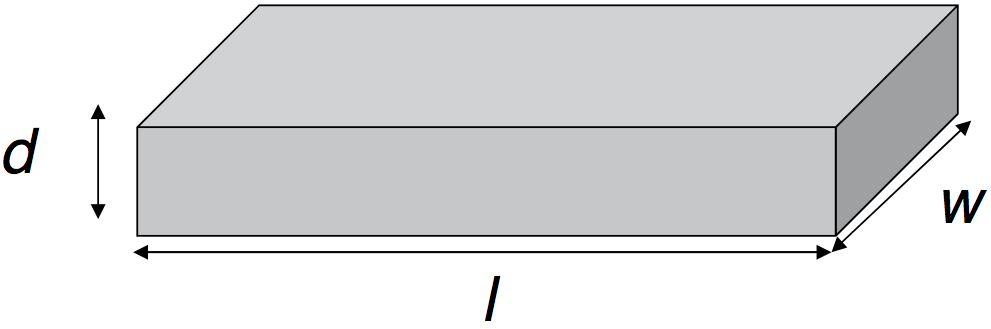
\includegraphics[width=0.3\textwidth]{pictures/widerstand.png}

\columnbreak

$R=\rho\frac{l}{w*d}$ \\
$\rho$: Spezifischer Widerstand
\end{multicols} 

\subsection{Kondensatoren}
\subsubsection{Kapazitätswert}
\begin{multicols}{2}
	\begin{center}
		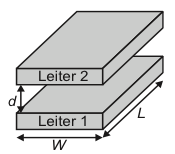
\includegraphics[width=0.15\textwidth]{pictures/kapazitaetswert}
	\end{center}
	\columnbreak

	\begin{equation*}
		C=\varepsilon_{r}*\varepsilon_{0}*\frac{W*L}{d}=\varepsilon_{r}*\varepsilon_{0}*\frac{A}{d}
	\end{equation*}
	mit $\varepsilon_{0}= 8.85 pF/m$
\end{multicols}


\subsubsection{Einschaltvorgang}
\input{idiotenseite/elektrotechnik/subsections/einschalt_kondensator}

\subsubsection{Ersatzschaltbild}
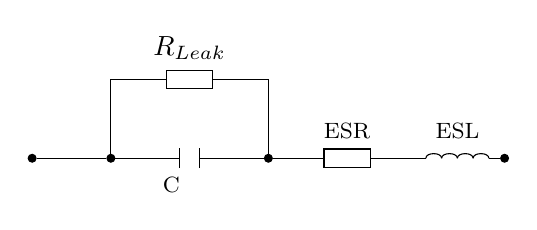
\begin{tikzpicture}

  \node (dot) at (1,1) [draw,circle,inner sep=1,fill]{};
  \node (dot2) at (2,1) [draw,circle,inner sep=1,fill]{};

  \node (c) at (3,1) [rectangle]{};
  \node (rleak) at (3,2)[draw,rectangle]{$~~~$};
  \node (dot3) at (4,1) [draw,circle,inner sep=1,fill]{};
  \node (esr) at (5,1)[draw,rectangle]{$~~~$};
  \coordinate (eslstart) at (6,1);
  \coordinate (eslend) at (6.8,1);
  \node (esl) at (6,1)[rectangle]{};
  \node (dot4) at (7,1) [draw,circle,inner sep=1,fill]{};

  \draw (dot) -- (dot2) -- (c) -- (dot3) -- (esr) -- (eslstart) (eslend) -- (dot4);
  \draw (dot2) |- (rleak) -| (dot3);

  \draw (c.south west) -- (c.north west);
  \draw (c.south east) -- (c.north east);

 \begin{scope}[out=90,in=90]
   \foreach \x in {0,0.2,0.4,0.6}
      \draw (eslstart)++(\x,0) to ++(0.2,0);
 \end{scope}

 \draw (rleak.north) node[above]{$R_{Leak}$};
 \draw (esr.north) node[above]{\footnotesize ESR};
 \draw (esl.north) node[above right]{\footnotesize ESL};
 \draw (c.south) node[below left]{\footnotesize C};


\end{tikzpicture}


\subsection{Induktivitäten/Spulen}
\begin{multicols}{2}
	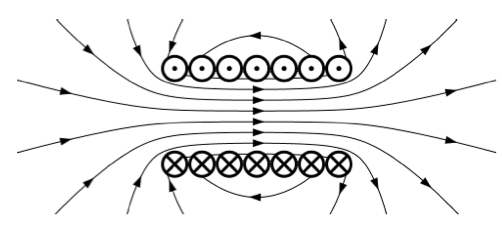
\includegraphics[width=0.4\textwidth]{pictures/induktivitaet}
	\columnbreak
	\begin{itemize}
  		\item Eine Änderung des elektrischen Stromes erzeugt ein Magnetfeld, das der
  			Stromänderung entgegenwirkt
  		\item Masseinheit Henry : $H=\frac{AS}{Vm}$
	\end{itemize}
	\begin{align*}
  		u_{i} &=-N\cdot\frac{d\Phi}{dt}\\
  		L &=\frac{N\cdot\Phi}{I} \\
  		L &=N^2\cdot\frac{\mu_{0}\mu_{r}A}{2\pi r} & \text{Ringspule} \\
  		L &=N^2\cdot\frac{\mu_{0}\mu_{r}A}{l} & \text{Zylinderspule}
	\end{align*}
\end{multicols}

\subsubsection{Einschaltvorgang}
\input{idiotenseite/elektrotechnik/subsections/einschalt_spule}

\subsubsection{Ersatzschaltbild}
\begin{tikzpicture}

  \node (dot) at (1,1) [draw,circle,inner sep=1,fill]{};
  \node (dot2) at (2,1) [draw,circle,inner sep=1,fill]{};

  \node (c) at (3.5,2) [rectangle]{};
  \node (l) at (3,1)[rectangle]{};
  \coordinate (lstart) at (2.6,1);
  \coordinate (lend) at (3.4,1);
  \node (rcu) at (4,1)[draw,rectangle]{$~~~$};
  \node (dot3) at (5,1) [draw,circle,inner sep=1,fill]{};
  \node (dot4) at (6,1) [draw,circle,inner sep=1,fill]{};

  \draw (dot) -- (dot2) -- (lstart) (lend) --(rcu)  -- (dot3)  -- (dot4);
  \draw (dot2) |- (c) -| (dot3);

  \draw (c.south west) -- (c.north west);
  \draw (c.south east) -- (c.north east);

 \begin{scope}[out=90,in=90]
   \foreach \x in {0,0.2,0.4,0.6}
      \draw (lstart)++(\x,0) to ++(0.2,0);
 \end{scope}

 \draw (rcu.south) node[below]{\footnotesize $R_{Cu}$};
 \draw (l.south) node[below]{\footnotesize L};
 \draw (c.north) node[above]{\footnotesize $C_p$};

\end{tikzpicture}


